\documentclass[a4paper, 12pt]{article}
\usepackage[T1]{fontenc}
\usepackage[brazilian]{babel}
\usepackage[utf8]{inputenc}
\usepackage[dvips]{geometry}
\geometry{a4paper,nohead,left=1in,right=1in,top=3cm,bottom=3cm}

\usepackage[fleqn]{amsmath}
\usepackage{indentfirst}
\usepackage{graphicx}
\usepackage[colorinlistoftodos]{todonotes}
\usepackage[colorlinks,pagebackref,hyperindex]{hyperref}
\usepackage[portuguese,linesnumbered,commentsnumbered,ruled,vlined]{algorithm2e}
\usepackage{setspace}
\usepackage{mathtools}	
\usepackage{subfigure}
\DeclarePairedDelimiter\ceil{\lceil}{\rceil}
\DeclarePairedDelimiter\floor{\lfloor}{\rfloor}
\usepackage{amsmath}
\usepackage{adjustbox}

\hypersetup{pdfpagelayout=SinglePage, % ou TwoPageLeft
    	colorlinks=true,       		% false: boxed links; true: colored links
        	linkcolor=black,          	% color of internal links
        	citecolor=black,        		% color of links to bibliography
        	filecolor=magenta,      		% color of file links
    		urlcolor=blue,
    		bookmarksdepth=4}
% Definindo novas cores
\definecolor{verde}{rgb}{0,0.5,0}
% Configurando layout para mostrar codigos C++
\usepackage{listings}
\lstset{
  language=C++,
  basicstyle=\ttfamily\small, 
  keywordstyle=\color{blue}, 
  stringstyle=\color{verde}, 
  commentstyle=\color{red}, 
  extendedchars=true, 
  showspaces=false, 
  showstringspaces=false, 
  numbers=left,
  numberstyle=\tiny,
  breaklines=true, 
  backgroundcolor=\color{green!10},
  breakautoindent=true, 
  captionpos=b,
  xleftmargin=0pt,
}
\begin{document}
%\maketitle
\onehalfspace
\begin{titlepage}
	\begin{center}
		\large{Universidade Federal de Minas Gerais\\
			Instituto de Ciências Exatas\\
			Departamento de Ciência da Computação\\
		}

\vspace{70pt}

      
        \vspace{85pt}
        
		\textbf{\huge{Computação Natural\\}}
		\large{\textbf{Trabalho 2:
        		Colônia de Formigas}}
		\vspace{160pt}
		
	\end{center}
	
	\begin{flushleft}
		\begin{tabbing}
			Aluna:\qquad\qquad\= Larissa Fernandes Leijôto\\
			Email:\qquad\qquad larissaleijoto@ufmg.br\\
			Professor:\> Gisele Lobo Pappa\\
		
	\end{tabbing}
		  
	\end{flushleft}
	
	\begin{center}
		\vspace{\fill}
		Belo Horizonte, \\22 de dezembro de 2015
	\end{center}
\end{titlepage}
%%%%%%%%%%%%%%%%%%%%%%%%%%%%%%%%%%%%%%%%%%%%%%%%%%%%%%%%%%%%%%%%%%%%%%%%%%%%%%%%%%%%%%%%%%%%%%%%%%%%%%%%%%%%% 
\newpage
\tableofcontents
\thispagestyle{empty}

\newpage
\pagenumbering{arabic}

\section{Introdução}
Otimização por colônia de formigas(ACO, \textit{Ant Colony Optimization}) é uma metaheurística que compõe a classe de algoritmos que são baseados em inteligência de enxames. O ACO é utilizado para encontrar soluções aproximadas em problemas de otimizações cujo as soluções exatas são impossíveis encontrar em tempo polinomial. Por isso, seu uso é indicado para encontrar a solução para o problema de encontrar o caminho máximo em uma grafo. O ACO e inspirado em como as formigas se comportam no meio ambiente, seu comportamento é baseado na comunicação através de uma substância denominada feromônio. 

Quando uma formiga encontra comida ela deixa um rastro no caminho de volta para a colônia, e esse rastro é seguido por outras formigas que o quando elas voltam à colônia. Quando o alimento acaba, as trilhas não são mais modificadas pelas formigas que retornam, e o cheiro se perde. Esse comportamento ajuda as formigas a se adaptarem à mudanças em seu meio. Quando um caminho estabelecido para uma fonte de comida é bloqueado por um novo obstáculo, as formigas o deixam para explorar novas rotas. Se bem sucedida, a formiga retorna e marca um novo rastro para a rota mais curta. Trilhas bem sucedidas, são seguidas por mais formigas, e cada uma o reforça com mais feromônio.

Esse comportamento das formigas é simulado no computador por meio de uma população de formigas, onde cada uma é uma possível solução para o problema abordado. O ambiente que será percorrido por elas é representado por meio de uma matriz que possui uma concentração inicial de feromônio. A medida que as formigas vão percorrendo o seu caminho ela deixa uma taxa constante de feromônio que é acumulada à que já estava lá. Esse feromônio é utilizado para marcar caminhos em que as formigas passam com mais frequência, ou seja, quanto maior a concentração de feromônio, mais formigas percorreram o caminho, e quanto mais alto, maior será a probabilidade de novas formigas passarem por ele. Cada formiga guarda o seu caminho, e consequentemente a avaliação dele, que é feita por meio da soma das distâncias das arestas que o compõe.

\section{Modelagem e solução proposta}

Nesta seção será discutida a modelagem das formigas, bem como a sua avaliação. Apresentaremos também como os parâmetros do algoritmo foram utilizados e quão sensível o programa é a eles.
O problema abordado será o de encontrar o caminho máximo entre dois vértice de um grafo. Dados vértices i e f, sendo i o vértice inicial e f o vértice final de um grafo direcionado com distâncias positivas nas aresta,o problema consiste em encontrar um caminho máximo de i a f.

\subsection{O algoritmo de colônia de formigas}
 Formigas artificiais são heurísticas construtivas. Elas constroem soluções de forma probabilística utilizando duas informações: A trilha de feromônio que muda dinamicamente durante a execução do programa de modo a refletir a experiência já adquirida durante a busca; A informação heurística especifica do problema a ser resolvido. O algoritmo implementado neste trabalho segue o fluxo básico de um algoritmo de otimização por colônia de formigas. O pseudo-código do algoritmo pode ser visto no Algoritmo \ref{alg:algoritmo1}.


\begin{algorithm}[h]
\SetAlgoLined
\Entrada{Conjunto de vértices}
\Saida{Melhor caminho}

Inicializar formigas; \\
\Repita{(Alcançar critério de convergência)}{
calcular probabilidades\;
evaporar feromônio das arestas\;
atualizar feromônio das arestas\;
atualizar fomigas\;
}
\caption{Esboço do algoritmo implementado}
\label{alg:algoritmo1}
\end{algorithm}
\setlength{\parskip}{0.0cm}


\subsection{Implementação}
O algoritmo de otimização por colônia de formigas foi implementado na linguagem C++ com dependência das bibliotecas standards do c++11(iostream, fstream, string, vector, e chrono). 


\subsubsection{Formiga}
Para a representação das formigas foram utilizados \textit{structs} que são compostos pelo caminho que as formigas trilham e pelas distância percorrida por elas. Para a representação do caminho foi utilizado um vetor denominado \textit{path}, assim cada formiga possuirá seu próprio caminho de acordo com as probabilidades de transição. A variável \textit{distance} é a soma das distâncias das arestas que a formiga esteve.

\begin{lstlisting}
struct Ant 
{
  double distance;
  vector<int> path;
};
\end{lstlisting}

\subsubsection{Distâncias}
Para a representação das distância entre a cidades utilizamos uma matriz de adjacência, cuja a linha e a coluna representa a distância entre as cidades.
\begin{lstlisting}
vector<vector<double>> adjacencies;
\end{lstlisting}

\subsubsection{Feromônio}
Para a representação do ambiente que as formigas circulam, utilizamos uma matriz de feromônio, que são depositados pelas formigas a medida que elas passam, sendo assim a posição da matriz contém o feromônio associado a ela.

\begin{lstlisting}
vector<vector<double>> pheromone;
\end{lstlisting}

\subsubsection{Probabilidades}

A probabilidade da formiga k que está no vértice i escolher a cidade j é dada pela regra demonstrada na Equação \ref{eq1}.

\begin{equation}
{p^k}_{ij} = \frac{(\tau_{ij})^\alpha(\eta_{ij})^\beta}{\sum(\tau_{ij})^\alpha(\eta_{ij})^\beta}
\label{eq1}
\end{equation}

\begin{itemize}
\item  $\tau_{ij}$é feromônio associado a aresta (i,j).\\
\item $\alpha$ e $\beta$ são parâmetros para determinar a influência do feromônio e da informação heurística.\\
\end{itemize}

Associada a aresta (i, j) existe um valor heurístico $\eta_{ij}$ dado pela Equação \ref{eq2} que representa a atratividade da formiga visitar a cidade i depois de visitar a cidade j. O valor $\eta_{ij}$ é inversamente proporcional a distância $d_{ij}$ entre as cidades i e j. 

\begin{equation}
\eta_{ij} =\frac{1}{d_{ij}}
\label{eq2}
\end{equation}

\subsubsection{Métodos importantes}

\begin{lstlisting}
void antOptimization(int , int, int);
void MakeGraphDistances(vector<vector<double>>&);
void init_ant(vector<Ant>&, int );
void seed_initial_pheromone(vector<vector<double>>&, 
     vector<vector<double>>&);
void build_solution(vector<Ant> &, vector<vector<double>> &, 
     vector<vector<double>> &);
void pheromone_evaporates(vector<vector<double>> &);
void update_pheromone(vector<Ant> &, vector<vector<double>> &);
\end{lstlisting}

\begin{itemize}
\item \textbf{antOptimization:} Método principal do algoritmo implementado, realiza a chamadas de todos os outros métodos implementado no programa
\item \textbf{MakeGraphDistances:} Monta a matriz de adjacências para ser usada pelo algoritmo.
\item \textbf{init\_ant:} Inicaliza as formigas e as trilhas delas de forma aleatória
\item \textbf{seed\_initial\_pheromone:} Inicializa o feromônio baseado em uma fórmula para o cálculo do mesmo.
\item \textbf{build\_solution:} Constrói a trilha que será percorrida.
\item \textbf{pheromone\_evaporates:} Subtrai uma taxa constante da matriz de feromônio
\item \textbf{update\_pheromone:} Atualiza o feromônio de cada cidade de acordo com os caminhos que já foram percorridos pelas formigas.
\end{itemize}



\section{Arquivos, compilação e execução}
\subsection{Arquivos}
\begin{itemize}
\item \textbf{main.cpp:} Arquivo principal que realiza a chamadas dos principais métodos.
\item \textbf{util.cpp:} Métodos úteis que foram utilizados na implementação do algoritmo.
\item \textbf{database.cpp:} Arquivo utilizado para a leitura da base de dados.
\item \textbf{util.h:} Header da classe util
\item \textbf{database.h:} Header da database
\item \textbf{antOptimization.cpp} Arquivo princial onde é implementado o alogritmo de colônia de formigas
\item \textbf{antOptimization.h} Header do algoritmo de colônia de formigas
\end{itemize}

\subsection{Compilação}
A compilação do programa pode ser feito por meio de um Makefile contido na pasta raiz do trabalho. Outro Makefile que pertence a pasta src é executado, assim que o primeiro Make é acionado. Portanto, não é necessário executá-lo uma vez que, sua execução é a partir do que está contido na pasta raiz.

\begin{enumerate}
\item[-] $tp2-naturalComputing/make$
\end{enumerate}


\subsection{Execução}
Para que o programa seja executado é necessário o seguinte comando:

\begin{enumerate}
\item[-] $bin/antOptimization [nAnts, nIteration, evaporationRate, input/File]$
\end{enumerate}

\section{Experimentos}
Os experimentos foram executados em um computador com processador Intel Core I5 com 1.70GHz, memória DDR3 de 8 GB e sistema operacional Ubuntu versão 14.04.3 LTS.


\subsection{Metodologia}
O algoritmo implementado é influenciado pelos parâmetros apresentado na Tabela \ref{tab1}. Por opção de tempo de processamento o algoritmo foi implementado de forma que pudesse gerar soluções inválidas. Isso possibilitou que ele achasse soluções mais rápido do que a abordagem que utiliza \textit{backtraking} para gerar somente soluções válidas. Para a análise do resultado foi criado um scrip para variar o número de formigas, a quantidade de iterações e a taxa de evaporação. A semente utilizada para essa variação foi 1834, e a configuração de parâmetros que obteve o melhor resultado foi usado para executar o algoritmo na fase final. Essa abordagem foi adota para que seja possível analisarmos a convergência do algoritmo e a significância do resultado. Para as três entradas definimos que o limite de iterações seria de 10 a 500, o limite de formigas dependeria da quantidade de vértice que cada entrada possui e a taxa de evaporação foi variada em um intervalo de 0.1 a 0.9. As constantes associada ao algoritmo foram definidas utilizando a Entrada 2, onde foram realizados uma teste com diversas variações delas. 

\begin{table}[!htb]
\centering
\caption{Parâmetros}
\label{tab1}
\begin{tabular}{|l|l|}
\hline
Parâmetros                               \\\hline
Influência do feromônio                  \\
Influência da visibilidade               \\
Número de formigas                       \\
Constante de acréscimo de feromônio      \\
Constante de inicialização do feromônio  \\\hline
\end{tabular}
\end{table}

\newpage

\section{Resultados}
Para determinar a significância dos resultados o algoritmo foi executado 30 vezes para as três entradas disponíveis. Utilizando todas as execuções foi calculada a média, a variância e o desvio padrão. O resultado para essas métricas é apresentado na tabela \ref{estatisticas}.

\begin{table}[!htb]
\centering
\caption{Métricas}
\label{estatisticas}
\begin{tabular}{|l|l|l|l|}
\hline
              & Entrada 1 & Entrada 2 & Entrada 3   \\\hline
Média         & 960.76    & 166.26    &  9524.40    \\
Desvio Padrão & 5.50      & 1.36      &  272.21     \\
Variância     & 30.32     & 1.85      &   74101.28   \\
Max           & 973       & 167       &   9753        \\
Min           & 953       & 163       &   8941      \\\hline
\end{tabular}
\end{table}



Observando uma execução de um dos experimentos realizados com cada entrada, podemos perceber que o algoritmo implementado converge rapidamente para uma solução. No experimento demostrado na Figura \ref{fig:fig1}  o algoritmo convergiu para um ótimo local, isso ocorreu também nos outros 30 experimentos. Sendo assim, em nenhuma das execuções nessa entrada o algoritmo conseguiu encontrar o ótimo, mas apesar disso em algumas execuções ele conseguiu chegar bem próximo, pois o máximo alcançado foi 973 e o valor ótimo informado é de 990.



\begin{figure}[!htb]
\centering
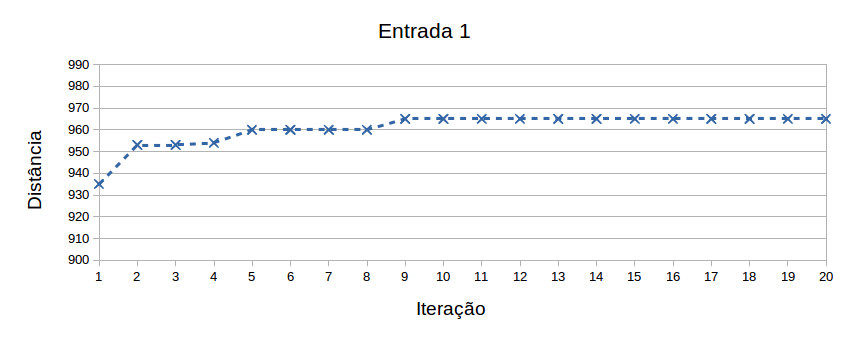
\includegraphics[scale=0.64]{entrada1.png}
\caption{Demostração de uma execução para a primeira entrada.}
\label{fig:fig1}
\end{figure}

No experimento demostrado na Figura \ref{fig:fig2} podemos observar que o algoritmo novamente convergiu muito rápido, mas como essa entrada é relativamente mais fácil que a anterior podemos ver que ele chegou muito mais próximo do ótimo. O máximo alcançado foi de 167, sendo que a solução ótima é de 168.

\begin{figure}[!htb]
\centering
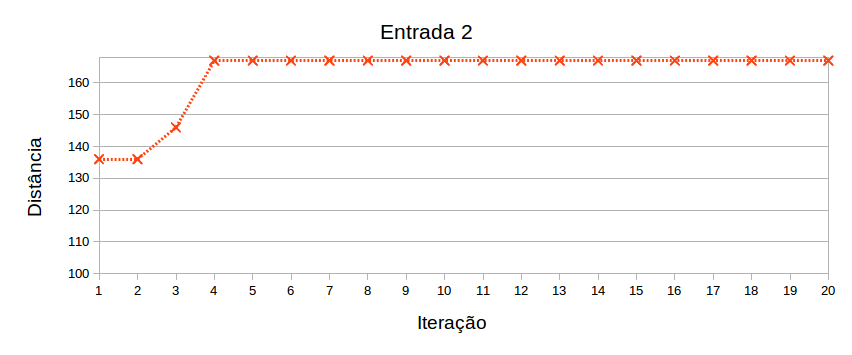
\includegraphics[scale=0.64]{entrada2.png}
\caption{Demostração de uma execução para a segunda entrada.}
\label{fig:fig2}
\end{figure}


O experimento realizado na ultima base seguiu o mesmo comportamento das anteriores, por isso pressupomos que o valor máximo encontrado seja um ótimo local. O valor máximo foi de 9753, e como nessa base nós não possuímos o ótimo não saberemos dizer o quão próximo a nossa solução ficou em relação a ele. Como mostrado na Tabela \ref{estatisticas} a variância entre as execuções foi muito alta indicando que o algoritmo poderia ter sido executado por mais iterações. Entretanto, como vimos executá-lo por mais iterações não necessariamente melhoraria o resultado, por isso achamos esse teste dispensável.


\begin{figure}[!htb]
\centering
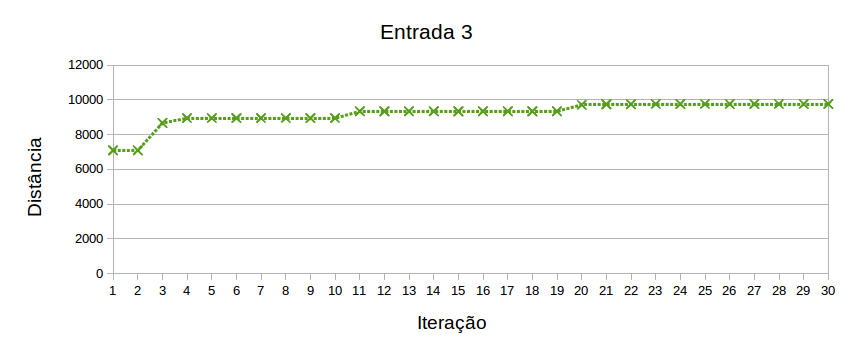
\includegraphics[scale=0.64]{entrada3.png}
\caption{Demostração de uma execução para a terceira entrada.}
\label{fig:fig3}
\end{figure}

\section{Conclusão}
Na implementação do algoritmo optamos por deixar ele gerar soluções inválidas, isso pelo fato dessa abordagem ser amplamente mais rápida que a que gera somente soluções válidas. Com os experimentos podemos concluir que a geração das soluções inválidas não acarretou prejuízos nas soluções que foram geradas. Como foi descrito na seção de resultado, as soluções não atingiram o ótimo esperado. Entretanto, para a Entrada 2 o algoritmo chegou muito próximo e para a Entrada 1 o fator de erro não foi grande. Na Entrada 3, vimos que a variância das execuções foi muito alta indicando que seriam necessárias uma maior quantidade de iterações para que ela diminuísse. Vimos também que aumentar a quantidade de iterações possivelmente não melhoraria o resultado, uma vez que ele já estava estacionado em uma solução a muitas iterações. Assim, concluímos que o algoritmo de colônia de formigas implementado cumpriu o seu papel, que é achar soluções próximas do ótimo para problemas de grande dificuldade.  


\end{document}